\par
\textsc{Gauss} sagt nun im Art. 6 (Werke X, 1, S. 222), dass man in \(k'=q^2/p^2\)
»statt \(t\) setzen könne
\begingroup\makeatletter\tagsleft@true\let\veqno\leqno\makeatother
\begin{equation*}
t'=\frac{\mathfrak p t+2\mathfrak q i}{2\mathfrak s it+\mathfrak r},\tag{22}
\end{equation*}
\endgroup
\noindent wo \(\mathfrak p,\mathfrak q,\mathfrak r,\mathfrak s\) beliebige, der Bedingung
\(\mathfrak p\mathfrak r+4\mathfrak q\mathfrak s=1\) genügende ganze reelle
Zahlen sind«, und untersucht weiterhin durch die Kettenbruchentwicklung von
(22), die ja die Zusammensetzung dieser Substitution aus den Fundamentalsubstitutionen \(t+2i,\ \frac1t\) liefert, das Verhalten von \(p(t)\) bei Anwendung von
(22). — Allgemeiner war es für \textsc{Gauss} auf Grund seiner zahlentheoretischen
Einsichten klar, dass sich aus den beiden Substitutionen \(t+i,\ \frac1t\) die allgemeine
Transformation (13) zusammensetzen lässt\footnote{Die weiter unten zu besprechende Aufzeichnung 6) aus dem Jahre 1805 gibt die Kettenbruchentwicklung einer beliebigen Substitution (13), die diese Zusammensetzung direkt liefert.}, und so lag es nahe, mit
Hilfe der Formeln (16), (17) das Verhalten der \(p,q,r\) bei den Transformationen
(13) zu untersuchen, und zwar in den sechs Fällen modulo 2, von
denen (22) denjenigen darstellt für den
\begingroup\makeatletter\tagsleft@true\let\veqno\leqno\makeatother
\begin{equation*}
\begin{pmatrix}\alpha&\beta\\\gamma&\delta\end{pmatrix}
\equiv\begin{pmatrix}1&0\\0&1\end{pmatrix}\pmod 2\tag{22a}
\end{equation*}
\endgroup
\noindent ist; man bezeichnet die Gesamtheit dieser Substitutionen mit F. \textsc{Klein} als
Hauptkongruenzgruppe zweiter Stufe. — Der Art. 7 (Werke X, 1, S. 224) gibt
in einer Tabelle das Resultat dieser Untersuchung und stellt auch gleich den
Zusammenhang zwischen den Transformationen (13) und der Äquivalenztheorie
der binären quadratischen Formen mit der Determinante \(-1\) heraus. Im
folgenden Art. 8 geht \textsc{Gauss} dann direkt darauf aus, auf Grund der Reduktionstheorie
dieser Formen die Funktionen \(p(t),q(t),r(t)\) durch solche darzustellen,
in denen \(t\) »\textls[100]{die einfachste Form}« hat. Man wird hiernach die
Reduktionstheorie der quadratischen Formen geradezu als eine der Wurzeln
bezeichnen müssen, aus denen bei \textsc{Gauss} die Theorie der Modulfunktion herauswächst.

Er bildet nämlich für \(t=g+hi\) die quadratische Form
\begingroup\makeatletter\tagsleft@true\let\veqno\leqno\makeatother
\begin{equation*}
\left(\frac1g,\ \frac hg,\ \frac{g^2+h^2}g\right)\tag{23}
\end{equation*}
\endgroup
\clearpage\SourceLeaf{184}\ArithmeticHead{99}{R}{Vc. THEORIE DER MODULFUNKTION.}
\HistoricalFoot{}{13\textsuperscript{*}}
\noindent mit der Wurzel \(ti\) und der Determinante \(-1\), und zwar zuerst für den Fall,
wo \(g,h\) rational sind, dann auch, wenn diese nicht rational sind, und bestimmt
durch den bekannten Reduktionsalgorithmus (\textit{Disqu. arithm.} Art. 171,
Werke I, S. 146) die äquivalente reduzierte Form \((a,b,c)\), deren Wurzel
dann jenen »einfachsten« Wert \(\frac{1+bi}a\) von \(t\) liefert. Bestimmt man dann »die
Transformation von (23) in \((a,b,c)\), so werden deren Elemente (ob sie gerade
oder ungerade) entscheiden, welche Funktion von \(\frac{1+bi}a\) mit der gegebenen
von \(t\) so zusammenhängt, dass die letztere in \(\varepsilon^H\sqrt{t\mathpunct{.}t'\mathpunct{.}t''\ldots}\) multipliziert werden
muss«. Dabei bedeuten \(\varepsilon\) eine achte Einheitswurzel \(\sqrt i\), \(t'i,t''i,\ldots\) die Wurzeln
der »benachbarten« quadratischen Formen, die beim Reduktionsalgorithmus auftreten,
und \(H\) eine durch eben diesen Algorithmus bestimmte ganze Zahl.

Die Herstellung des Zusammenhangs zwischen den verschiedenen Bestimmungen
des agM. vollzieht sich nun ohne jede Schwierigkeit\footnote{Wir benutzen im folgenden eine Betrachtung von L. v. \textsc{Dávid}, Mathem.-naturw. Berichte aus Ungarn 27, 1913, S. 164—171, Rendiconti di Palermo 35, 1913, S. 82—89.}. Die
Gleichung
\[
\begin{aligned}
a:b:\sqrt{a^2-b^2}&=p(t)^2:q(t)^2:r(t)^2\\
&=p(t')^2:q(t')^2:r(t')^2
\end{aligned}
\]
\noindent besteht für ein mit \(t\) durch die Transformation (13) verknüpftes \(t'\) dann und
nur dann, wenn
\begingroup\makeatletter\tagsleft@true\let\veqno\leqno\makeatother
\begin{equation*}
\begin{pmatrix}\alpha&\beta\\\gamma&\delta\end{pmatrix}
\equiv\begin{pmatrix}1&0\\0&1\end{pmatrix}\pmod 4\tag{24}
\end{equation*}
\endgroup
\noindent ist, d. h. für die Hauptkongruenzgruppe vierter Stufe. Das ergibt sich ohne
weiteres aus der Abhandlung des Handbuchs 16, Bb (1827), Werke III,
S. 478; daselbst ist nämlich gezeigt, dass, wenn \(t'\) mit \(t\) durch eine Substitution
(13) zusammenhängt, für die \(\alpha,\delta\equiv1\pmod4\), \(\beta,\gamma\) gerade sind,
\[
\frac{q(t')^2}{p(t')^2}=i^\gamma\frac{q(t)^2}{p(t)^2}
\]
\noindent gilt. Also bleibt \(k'\) für \(\gamma\equiv0\pmod4\) ungeändert; soll auch \(k\) ungeändert
bleiben, so muss auch \(\beta\equiv0\pmod4\) sein\footnote{Vergl. \textsc{Geppert} a. a. O. \textsuperscript{83)}, § 30, S. 124ff.}. Dagegen ist \(k'^2=q(t)^4/p(t)^4\),
die Modulfunktion im engern Sinne, für die Substitutionen der Hauptkongruenzgruppe
zweiter Stufe (22) invariant. — Für die Hauptkongruenzgruppe
vierter Stufe (24) ergibt sich aus der Tabelle des Art. 7 (Werke X, 1, S. 224)
\clearpage\SourceLeaf{185}\ArithmeticHead{100}{L}{L. SCHLESINGER, ÜBER GAUSS’ FUNKTIONENTHEORETISCHE ARBEITEN.}
\[
\begin{aligned}
p(t')^2&=(\gamma it+\delta)p(t)^2,\\
q(t')^2&=(\gamma it+\delta)q(t)^2,
\end{aligned}
\]
\noindent also wenn
\[
a=(\mu)\mathpunct{.}p(t')^2,\quad b=(\mu)\mathpunct{.}q(t')^2
\]
\noindent gesetzt wird, durch Vergleichung mit
\[
a=M(a,b)p(t)^2,\quad b=M(a,b)q(t)^2,
\]
\[
(\mu)=\frac{M(a,b)}{\gamma it+\delta},
\]
\noindent d. h. mit Rücksicht auf die Gleichung (18)
\begingroup\makeatletter\tagsleft@true\let\veqno\leqno\makeatother
\begin{equation*}
\begin{gathered}
\frac1{(\mu)}=\frac\delta{M(a,b)}+\frac{\gamma i}{M(a,\sqrt{a^2-b^2})},\\
\delta\equiv1,\ \gamma\equiv0\pmod4,
\end{gathered}\tag{25}
\end{equation*}
\endgroup
\noindent was den in der Tagebuchnotiz 109. angezeigten Zusammenhang zwischen den
verschiedenen Bestimmungen des agM. darstellt. Wir bemerken, dass sich
diese allgemeine Formel im Nachlasse von \textsc{Gauss} nicht vorfindet, aber die
Tagebuchnotiz 109. verbürgt, dass \textsc{Gauss} sie 1800 entdeckt hat. Wenn \(a>b\)
reell positiv und \(c>0\) sind, so sind die positiven Werte \(M(a,b),M(a,c)\) zusammengehörig,
also \(t=M(a,b)/M(a,c)\) positiv; entsteht nun, wie \textsc{Gauss} im
Art. 3 von 3) andeutet (vgl. oben S. 94), \((\mu)\) dadurch, dass etwa zuerst bei
der Bildung von \(b_n\) der negative Wert der Quadratwurzel gewählt wird, während
man vom \(k=n+1\) ab für \(b_k\) wieder denjenigen Wert der Quadratwurzel
nimmt, der dem entsprechenden \(a_k\) am nächsten liegt (so verfährt \textsc{Gauss} in
dem a. a. O. gegebenen Beispiel, Werke X, 1, S. 219), so ergibt die Tabelle
des Art. 7, dass das entsprechende \(t'\) den Wert
\[
t'=\frac t{1+2^{n+1}it}
\]
\noindent besitzt (vergl. den Art. 12 der Aufzeichnung 7) Werke III, S. 478, wo der
Fall \(n=0\) erörtert ist\footnote{Vergl. auch \textsc{Geppert}, a. a. O. \textsuperscript{83)}, S. 139, 140.}), man hat also \(\gamma=2^{n+1},\ \delta=1\), d. h. dieser Fall
ist in der Tat, wie \textsc{Gauss} sagt, »in der Form (10) begriffen«. Notwendig und
hinreichend für diese Form (10) ist, dass nicht nur \(\mu=M(a,b)\) und \(\lambda=M(a,c)\)
in dem Sinne zusammengehören, dass \(t=\mu/\lambda\) einen positiven reellen Teil hat,
sondern dass dies auch für \(t'=(\mu)/\lambda\) stattfindet; dann ist nämlich nach (25)
\clearpage\SourceLeaf{186}\ArithmeticHead{101}{R}{Vc. THEORIE DER MODULFUNKTION.}
\[
t'=\frac t{\delta+\gamma it},
\]
\noindent somit \(\alpha=1,\ \beta=0\), also, da \(\alpha\delta-\beta\gamma=1\) sein muss, \(\delta=1\)\footnote{Siehe v. \textsc{Dávid}, a. a. O., \textsc{Geppert}, Mathem. Annalen, 99, 1928, S. 166.}.

Aus der Reduktion von \(t\) auf die »einfachste Form« und der linearen
Transformation der \textls[100]{summatorischen Funktionen} \(p,q,r\) hat \textsc{Gauss}
(in der Aufzeichnung 4) Werke III, S. 386) die Aufgabe abgeleitet: »Sind
nämlich die Formen \((a,b,c),(A,B,C)\) äquivalent, so ist die Funktion \(f\)
in Betracht zu ziehen, wo \(f(t)\equiv f(u)\), sowohl wenn \(\frac{t-u}i\) ganze Zahl, als
wenn \(t=\frac1u\)«. Diese Funktion, die sich übrigens in keiner der Aufzeichnungen
1)—7) explizite angegeben findet, ist also nichts anderes als die
absolute Invariante der \textls[100]{Modulgruppe} aller linearen Substitutionen (13).
Sie wurde 1877 von \textsc{Dedekind}\footnote{R. \textsc{Dedekind}, \textsc{Crelles} Journal 83, 1877, S. 265; \textsc{Dedekinds} Werke, I, 1930, S. 174, besonders S. 193.} unter ausdrücklicher Bezugnahme auf die
hier in Rede stehende Stelle des \textsc{Gaussschen} Nachlasses als Valenz eingeführt
und dann durch \textsc{Klein} in den Mittelpunkt seiner Theorie der Modulfunktion
gerückt. Dass diese Funktion \(f(t)\) jeden Wert einmal und nur einmal
annimmt, wenn \(ti\) z. B. auf die Wurzeln mit positivem Koeffizienten von \(i\)
der reduzierten Formen beschränkt wird, hat \textsc{Gauss} so ausgesprochen: »Jeder
Klasse entspricht dann ein \textls[100]{bestimmter} Wert von \(f\left(\frac{1+bi}a\right)\)«\footnote{Werke III, S. 386. \textsc{Gauss} schreibt daselbst \(f\left(\frac{\sqrt p+bi}a\right)\), indem er nämlich quadratische Formen mit der Determinante \(-p\) in Betracht zieht, während wir hier anschliessend an die Festsetzungen der Aufzeichnung 3) die Determinante \(-1\) zu Grunde legen.}.

Wie man sieht, ist damit das Fundamentaltheorem der Theorie der Modulfunktion
gewonnen; \textsc{Gauss} brauchte jetzt nur noch die Werte \(\frac{1+bi}a\) in der
Zahlenebene zu repräsentieren, um den Fundamentalbereich der Modulgruppe
oder der Funktion \(f(t)\) zu erhalten.

Diese geometrische Interpretation findet sich, wie es scheint, zum ersten
Male in der Scheda An, einem Oktavheftchen betitelt »Cereri, Palladi, Junoni
sacrum, Febr. 1805«, dem die Werke VIII, S. 103 auszugsweise abgedruckte
Notiz 6) entstammt. Auf S. 6 dieser Scheda steht zunächst die Formel
\[
\frac{[\alpha,\beta,\ldots,\nu]\theta+[\beta,\gamma,\ldots,\nu]i}
{-i[\alpha,\beta,\ldots,\mu]\theta+[\beta,\gamma,\ldots,\mu]},
\]
\clearpage\SourceLeaf{187}\ArithmeticHead{102}{L}{L. SCHLESINGER, ÜBER GAUSS’ FUNKTIONENTHEORETISCHE ARBEITEN.}
\noindent die für eine beliebige Substitution (13) der Modulgruppe die Kettenbruchentwicklung\footnote{Die Bezeichnung \([\alpha,\beta,\ldots,\nu]\) hat \textsc{Gauss} im Art. 27 der \textit{Disqu. arith.} (Werke I, S. 20) bei der Auflösung der unbestimmten Gleichung \(ax=by\pm1\) eingeführt, die Kettenbruchentwicklung für eine ganzzahlige lineare Substitution gibt er ausführlich in den Artikeln 188, 189 desselben Werkes (Werke I, S. 171—175) aus Anlass der Reduktionstheorie der quadratischen Formen mit positiver Determinante. Vergl. die Darstellung bei \textsc{Dirichlet-Dedekind}, \textit{Vorlesungen über Zahlentheorie} § 81, 3. Aufl. 1880, S. 195.}, und damit die Zusammensetzung aus den beiden Fundamentalsubstitutionen
\(t+i,\ \frac1t\) liefert, mit der Ausführung von zwei Beispielen, dann
folgt auf S. 7 die berühmte Figur, die Werke VIII, a. a. O. wiedergegeben
ist. Wir wollen diese Figur aber hier in Verbindung mit einigen sie umrahmenden
und einigen auf S. 8 der Scheda befindlichen Formeln, mit einer
durch eben diese Formeln gebotenen leichten Abänderung gegen die Zeichnung
in Werke VIII reproduzieren\begingroup\renewcommand{\thefootnote}{140a)}\footnote{Werke VIII sind die kleineren Kreise, die durch den Nullpunkt gehen, nur halb so gross, also um die Punkte \(\pm\frac i8\) als Mittelpunkte mit dem Radius \(\frac18\) gezeichnet. Dass unsere Zeichnung der Absicht von \textsc{Gauss} entspricht, geht aus den Formeln, besonders der Ungleichung [II] hervor, vergl. weiter unten im Text. — Wir haben der in der Handschrift nur skizzierten Figur die Beschriftung und die gestrichelt gezeichneten Linien hinzugefügt, von den letzteren kommen die Geraden \(y=\pm\frac12\) in einer späteren Zeichnung von \textsc{Gauss} (siehe die Figur 3) vor.}\addtocounter{footnote}{-1}\endgroup, weil erst diese Formeln deutlich erkennen
lassen, was \textsc{Gauss} im Auge hatte, als er jene Figur hinzeichnete. Es
heisst Scheda An, S. 7:
\[
\begin{array}{ll}
\text{»[I]}&y<2\\
{}\text{[II]}&y<2xx+2yy
\end{array}
\]
\begin{center}
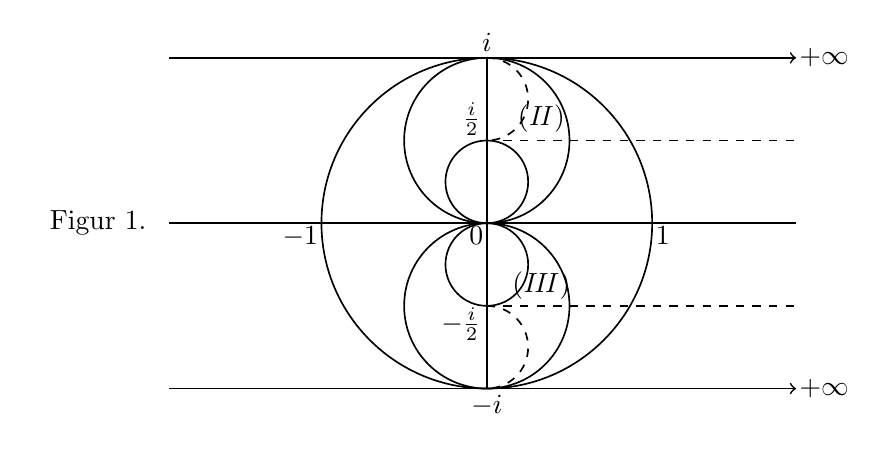
\begin{tikzpicture}[x=2.1cm,y=2.1cm,line width=.6pt]
\draw (0,0) circle[radius=1];
\draw (0,.5) circle[radius=.5];
\draw (0,-.5) circle[radius=.5];
\draw (0,.25) circle[radius=.25];
\draw (0,-.25) circle[radius=.25];
\draw (0,-1)--(0,1);
\draw (-1.92,0)--(1.87,0);
\draw[->] (-1.92,1)--(1.87,1);
\draw[->] (-1.92,-1)--(1.87,-1);
\draw[dashed] (0,1) arc[start angle=90,end angle=-90,radius=.25];
\draw[dashed] (0,-.5) arc[start angle=90,end angle=-90,radius=.25];
\draw[dashed] (0,.5)--(1.87,.5);
\draw[dashed] (0,-.5)--(1.87,-.5);
\node[above,inner sep=2pt] at(0,1){\(i\)};
\node[below,inner sep=2pt] at(0,-1){\(-i\)};
\node[below left,inner sep=1pt] at(0,0){\(0\)};
\node[below left,inner sep=1pt] at(-1,0){\(-1\)};
\node[below right,inner sep=1pt] at(1,0){\(1\)};
\node[left,inner sep=2pt] at(0,.63){\(\frac i2\)};
\node[left,inner sep=2pt] at(0,-.61){\(-\frac i2\)};
\node at(.33,.63){\(\mathit{(II)}\)};
\node at(.33,-.38){\(\mathit{(III)}\)};
\node[right,inner sep=1pt] at(1.87,1){\(+\infty\)};
\node[right,inner sep=1pt] at(1.87,-1){\(+\infty\)};
\node[left,inner sep=8pt] at(-1.92,0){Figur 1.};
\end{tikzpicture}
\end{center}
\[
\begin{array}{ll}
\text{[III]}&xx+y(y-1)\ \text{posit[iv]}\\
{}\text{[IV]}&(y+\tfrac12)^2+xx\geqq\tfrac14\text{«}
\end{array}
\]

\clearpage\SourceLeaf{188}\ArithmeticHead{103}{R}{Vc. THEORIE DER MODULFUNKTION.}
\noindent und Scheda An, S. 8: »Setzt man
\[
1+2e^{-\alpha\pi}+2e^{-4\alpha\pi}+\text{etc.}=(\alpha),
\]
\noindent so ist
\[
\begin{array}{rl}
1)&(\alpha+2ki)=(\alpha)\\[3pt]
2)&(\alpha+i)=2(4\alpha)-(\alpha)\\[3pt]
3)&\left(\frac1\alpha\right)=(\alpha)\sqrt\alpha\text{«.}
\end{array}
\]
